%!TeX root = ../My_thesis.tex


% .---|||___|||--- C H A P T E R ---|||___|||---. %
\chapter{Теоретическая часть работы}
% .---|||___|||--- C H A P T E R ---|||___|||---. %


% .---|||___|||--- S E C T I O N ---|||___|||---. %
\section{Этапы обработки естественного языка}
% .---|||___|||--- S E C T I O N ---|||___|||---. %


Как правило, в обработке текстов обычно выделяют следующие этапы~\cite[с.~9]{Batruha}:
\begin{enumerate}[1.]%
  \item Графематический анализ.
    Здесь осуществляется анализ на уровне символов, в том числе и токенизация, то есть разбиение набора символов (текста) на последовательность отдельных структурированных частей (слово, знак препинания, число, гиперссылка, адрес электронной почты и~т.\,д.).
  \item Морфологический анализ.
    Здесь происходит анализ на уровне слов (не токенов).
    Стоит выделить следующие процессы, проходящие на этом этапе:
    \begin{itemize}%
      \item Лемматизация
        "--- это нахождение нормальной (начальной) формы слова (леммы), к примеру, лемма у слова «сбегать» "--- «бегать».
        В японском это относится в основном к глаголам, так как у существительных, как правило, всего одна словоформа.
      \item Приписывание граммем.
        Граммемы "--- грамматическая характеристика, например, род, падеж, число.
        Граммемы могут помочь в разрешении неоднозначностей, которые возникают в морфологии.
    \end{itemize}
  \item Фрагментационный анализ.
    Осуществляется на уровне фраз, частей предложений. Этот этап неразрывно связан с синтаксическим анализом, а иногда и вовсе говорят о них, как об одном целом. Сюда, например, может входить обработка причастных или деепричастных оборотов.
  \item Синтаксический анализ.
    Осуществляется на уровне предложений.
    Здесь, как правило, строится дерево зависимостей одних слов от других, а также исключается морфологическая неоднозначность.
  \item Семантический анализ.
    Осуществляется на уровне всего текста.
    Самый сложный и неоднозначный из этапов, здесь появляется формальное представление смысла текста, как правило, в виде сементического графа.
    На сегодняшний день задачи семантического анализа чаще всего решаются искусственными нейронными сетями, о чём мы и поговорим далее.
\end{enumerate}


% .---|||___|||--- S E C T I O N ---|||___|||---. %
\section{Искусственные нейронные сети}
% .---|||___|||--- S E C T I O N ---|||___|||---. %


Вкратце, искусственная нейронная сеть (ИНС) представляет собой систему соединённых и взаимодействующих между собой простых нейронов. Каждый нейрон получает на вход несколько чисел (входные данные или же выходы других нейронов), суммирует эти числа с определёнными коэффициентами (нахождение оптимальных коэффициентов "--- обучение ИНС), после чего применяет к сумме функцию активации (любую нелинейную функцию) и передаёт результат на вход другому нейрону (или же на выход ИНС).

Существует большое множество различных архитектур ИНС (свёрточные, рекуррентные, рекурсивные, графовые и~т.\,д.), однако в данной работе будет сконцентрировано внимание на так называемых Transformer'ах, используемых, как правило, для языковой обработки, в частности для задач перевода и упрощения текстов.


% .---|||___|||--- S E C T I O N ---|||___|||---. %
\section{Какие модели используют для обработки естественных языков}
% .---|||___|||--- S E C T I O N ---|||___|||---. %


Существует большое количество моделей, использующихся для обработки естественных языков. Одними из наиболее популярных (до появления Transformer'ов) были следующие:
\begin{itemize}%
  \item Рекуррентные нейронные сети (RNN) (1982~г.):
    \begin{itemize}%
       \item Обработка последовательностей (например, текста).
       \item На каждый слой передаётся текущий элемент (слово) + результат предыдущего слоя.
       \item Причём есть обратные связи "--- поэтому рекуррентные.
       \item Очень медленные "--- из-за последовательной природы нельзя распараллелить.
     \end{itemize} 
  \item Долгая краткосрочная память (LTSM) (1997~г.):
    \begin{itemize}%
      \item Разновиднсть RNN с элементом «забывания».
      \item Ещё медленнее (из-за более сложного устройства каждого слоя модели).
    \end{itemize}
\end{itemize}

Для больших объёмов данных эти модели подходят не очень хорошо из-за своей последовательной природы обработки (требует огромных вычислительных ресурсов). На замену им пришли так называемые Transformer'ы (которые мы обсудим в следующем разделе).


% .---|||___|||--- S E C T I O N ---|||___|||---. %
\section{О модели Transformer}
% .---|||___|||--- S E C T I O N ---|||___|||---. %


Transformer "--- относительно новая (2017~г.) архитектура глубоких ИНС, разработанная в Google Brain.
Так же, как и рекуррентные ИНС (РНС), Transformer'ы предназначены для обработки последовательностей (к примеру, текста), то есть Transformer'ы относятся к sequence-to-sequence (seq2seq) моделям. В отличие от РНС, Transformer'ы не требуют обработки последовательностей по порядку, благодаря чему они распараллеливаются легче, чем РНС, и могут быстрее значительно обучаться.


% .---|||___|||--- S U B S E C T I O N ---|||___|||---. %
\subsection{Где применяются Transformer'ы}
% .---|||___|||--- S U B S E C T I O N ---|||___|||---. %


Используются Transformer'ы, например, в Яндексе (там его используют для лучшего ранжирования запросов, то есть поиск идёт не только по тексту, как обычной строке, но и по смыслу этого текста), во многих переводчиках (Яндекс, Google, DeepL и~т.\,д.), а также в GPT-3 "--- самой большой на сегодняшний день модели генерации текстов на английском языке.


% .---|||___|||--- S U B S E C T I O N ---|||___|||---. %
\subsection{Устройство Transformer'а}
% .---|||___|||--- S U B S E C T I O N ---|||___|||---. %


Transformer состоит из encoder'а и decoder'а. Encoder получает на вход последовательность слов в виде векторов (word2vec). Decoder получает на вход часть этой последовательности и выход encoder'а. Encoder и decoder состоят из слоев. Слои encoder'а последовательно передают результат следующему слою в качестве его входа. Слои decoder'а последовательно передают результат следующему слою вместе с результатом encoder'а в качестве его входа.

Каждый encoder состоит из механизма внимания (attention) (вход из предыдущего слоя) и ИНС с прямой связью (вход из механизма внимания). Каждый decoder состоит из механизма внимания (вход из предыдущего слоя), механизма внимания к результатам encoder'а и ИНС с прямой связью (вход из механизма внимания).


% .---|||___|||--- S U B S E C T I O N ---|||___|||---. %
\subsection{Механизм внимания}
% .---|||___|||--- S U B S E C T I O N ---|||___|||---. %


Каждый механизм внимания параметризован матрицами весов запросов $W_{Q}$, весов ключей $W_{K}$, весов значений $W_{V}$. Для вычисления внимания входного вектора $X$ к вектору $Y$, вычисляются вектора $Q=W_{Q}X$, $K=W_{K}X$, $V=W_{V}Y$. Эти вектора используются для вычисления результата внимания по формуле~\eqref{scaled-dot-product-attention}.

Если коротко, то внимание устанавливает взаимоотношения слов в предложении. Оно показывает нам насколько важен каждый элемент (по отдельности).
\begin{equation}\label{scaled-dot-product-attention}%
  \operatorname{Attention}(Q, K, V) = \underbrace{
    \operatorname{softmax}\left(
      \frac{QK^T}{\sqrt{d_k}}
    \right)
  }_{\text{scores}}
  V,
\end{equation}
где
\begin{itemize}%
  \item scores «оценивают» важность элементов (там лежат значения от 0 до 1).
  \item $Q$ (Query), $K$ (Key), $V$ (Value) "--- матрицы входных элементов.
  \item $d_k$ "--- нижняя размерность одной из этих матриц (длина части embedding'а).
\end{itemize}


% .---|||___|||--- S U B S E C T I O N ---|||___|||---. %
\subsection{MultiHead Attention}
% .---|||___|||--- S U B S E C T I O N ---|||___|||---. %


«Сердце» Transformer'ов "--- MultiHead Attention.
Несколько слоёв внимания позволяют «следить» за разными частями входной последовательности (независимо от других).
Добавляя больше этих слоёв, мы «следим» за бóльшим количеством частей последовательности.
\begin{equation}\label{multihead-attention-mechanism}%
  \operatorname{MultiHead}(Q, K, V) = \operatorname{Concat}\left(\operatorname{head}_1, \ldots, \operatorname{head}_h \right) W_0,
\end{equation}
где
\begin{itemize}%
  \item $\operatorname{head}_i = \operatorname{Attention}(QW_i^Q, KW_i^K, VW_i^V) $.
  \item $W_i$ "--- матрицы коэффициентов для обучения.
\end{itemize}


% .---|||___|||--- S U B S E C T I O N ---|||___|||---. %
\subsection{Positional Encoding}
% .---|||___|||--- S U B S E C T I O N ---|||___|||---. %


Так как в Transformer'е нет ни рекурренции (recurrence), ни свёртки, нам нужно что-то, что будет использовать порядок элементов в последовательности.
\begin{equation}\label{positional-encoding}%
  PE(p, 2i) = \sin\left( \frac{p}{10\,000^{2i / d_{\text{model}}}} \right),
\end{equation}
\begin{equation}\label{positional-encoding-2}%
  PE(p, 2i + 1) = \cos\left( \frac{p}{10\,000^{(2i + 1) / d_{\text{model}}}} \right),
\end{equation}
где
\begin{itemize}%
  \item $p$ (position) "--- позиция,
  \item $i$ (dimension) "--- размер предложения.
\end{itemize}


% .---|||___|||--- S U B S E C T I O N ---|||___|||---. %
\subsection{Обзор архитектуры Transformer'а}
% .---|||___|||--- S U B S E C T I O N ---|||___|||---. %


В оригинальной статье~\cite{Transformer2019} представлена следующая архитектура Transformer'а (см.~\firef{transformer-architecture}).
\begin{figure}[H]%
  \centering
  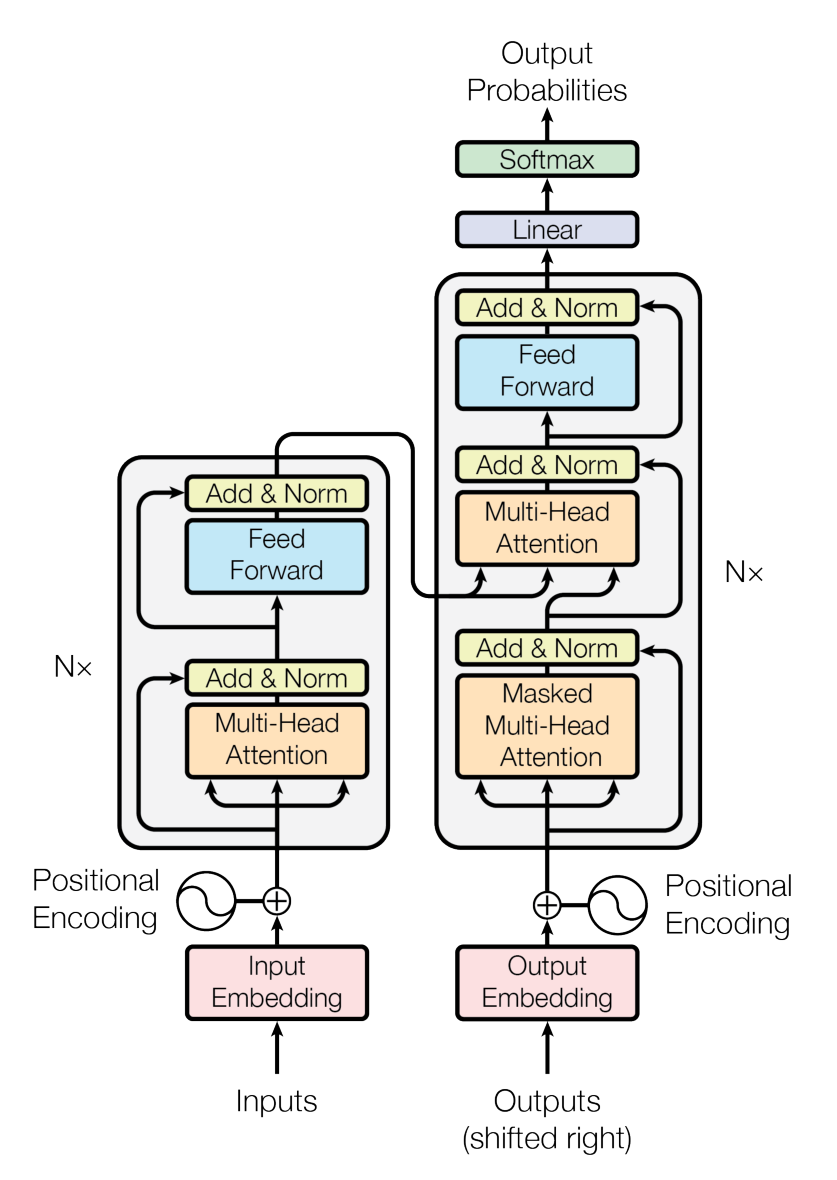
\includegraphics[width=0.5\textwidth]{transformer-architecture.png}
  \caption{Архитектура Transformer'а}
  \label{transformer-architecture}
\end{figure}

На~\firef{transformer-architecture} мы видим, что входные данные превращаются в эмбеддинги, после чего к ним суммируются positional encoding, после чего результат этой операции прогоняется через механизм MultiHead Attention, и, в итоге, через линейный слой со слоем Softmax мы получаем выходные вероятности элементов (слов в предложении).


% .---|||___|||--- S U B S E C T I O N ---|||___|||---. %
\subsection{Верхнеуровневый взгляд на Transformer}
% .---|||___|||--- S U B S E C T I O N ---|||___|||---. %


Какой высокоуровневый смысл несут encoder и decoder? Encoder представляет собой модель, «изучающую» исходный язык, его контекст (какие слова встечаются рядом в предложении, как следуют предложения друг за другом). То есть обучая encoder, мы обучаем модель «понимать» язык. Decoder же, в свою очередь, учится превращать контекст, полученный encoder'ом в какой-то осмысленный набор слов (в том числе и на другом языке). Иными словами, encoder получает информацию о предложениях, а decoder превращает эту информацию во что-то полезное (переведённое предложение, упрощённый текст, ответ на вопрос пользователя и т.д.)


% .---|||___|||--- S U B S E C T I O N ---|||___|||---. %
\subsection{Как encoder учится понимать контекст}
% .---|||___|||--- S U B S E C T I O N ---|||___|||---. %


Чтобы научить encoder понимать смысл текста на каком-либо языке, нужно его каким-то образом обучить (предоставить данные для обучения).
Отличная новость заключается в том, что данные для обучения можно получить относительно несложно, причём в очень больших объёмах.
В модели BERT~\cite{BERTmodel}, к примеру, сделали следующее: для большого набора языков выгрузили все статьи википедии для каждого из них.
После этого процесс обучения заключается в том, чтобы передавать encoder'у предложения, но не в исходном виде, а с замаскированными словами (вспомним маску, о которой мы говорили ранее), чтобы encoder пытался угадать, какое слово должно стоять в предложении.
Тоже самое делается и с предложениями "--- модели подаются 2 предложения, и она должна определить, следует ли оно предложение за другим.
Вся прелесть в том, что весь этот процесс обучения не нуждается в ручной обработке "--- маскировка случайных слов и подставление двух случайных предложений реализуется программно, причём довольно просто.

После чего эти большие объёмы данных прогоняются через encoder, обучая его, а на выходе мы получаем модель, имеющую довольно обширное знание о законах языка, о том, как строятся слова в предложениях, а также как строятся сами предложения. Далее нужно лишь дообучить decoder для решения нужной нам задачи (fine-tuning), что можно сделать даже на относительно небольшом массиве данных. В итоге мы получаем модель, превосходящую современные решения в мире NLP.
